\section{Auswertung}
\label{sec:Auswertung}

%\begin{figure}
%  \centering
%  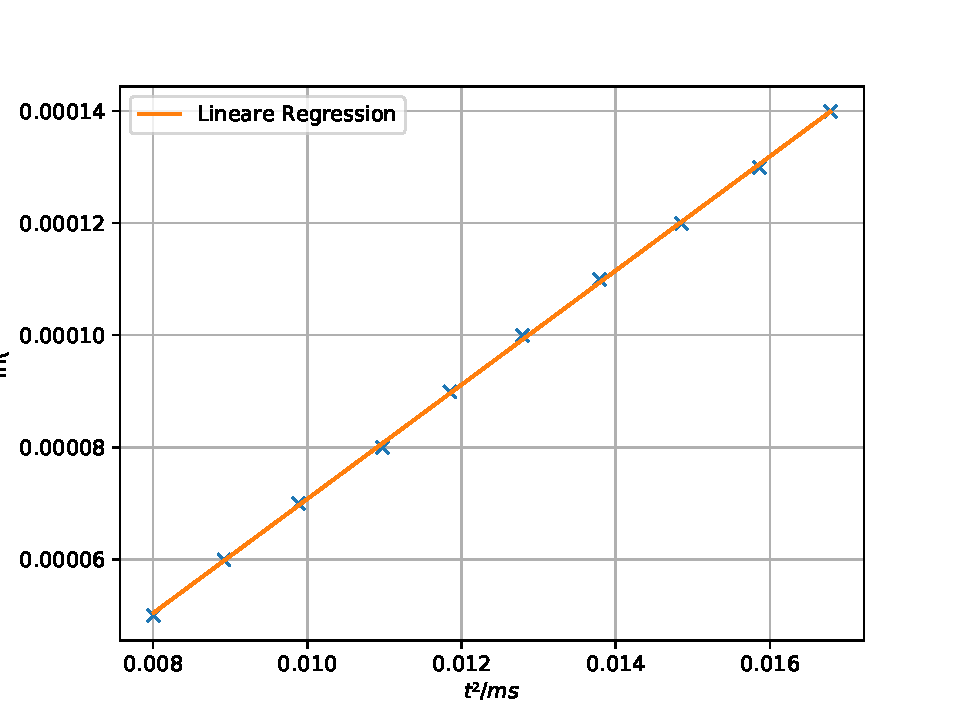
\includegraphics{Graphibitte.pdf}
%  \caption{Plot.}
%  \label{fig:plot}
%\end{figure}

%Einheiten: \SI{3}{\newton\s}
%1,41 \cdot \cramped{10^{-3}} ~s  für hochzahlen

%\begin{table}
%  \centering
%  \caption{Tabelle für a)Erste Bestimmung der Zeitkonstanten}
%  \label{Tab1}
%    \begin{tabular}{c c}%c zeigt die anzahl der Spalten
%      \toprule
%      Spannung $U_c$ &Zeit $t$\\% \\ werden benötigt um die Zeile zu Beenden
%      mV&ms\\% & Zeichen grenzen die Zahlen voneinander ab.
%      \midrule
%      \midrule
%        %\input{tab1.txt}% Die Tabelle ist hier ausgelagert. Sie kann aber auch genausogut hier eingefügt werden.
%          0,000 &     752\\
%          0,400 &     440\\
%          0,800 &     448\\
%      \bottomrule
%    \end{tabular}
%\end{table}

%\begin{table}
%    \centering
%    \caption{Messwerte für die Beta-Strahlung.}
%    \label{Tabg}
%    \sisetup{table-format=1.2}
%    \begin{tabular}{S S[table-format=2.2] S } %3 ziffern vom kommer, zwei danach, geht hiter jedes s
%      \toprule
%      %{$D$/cm}& \multicolumn{5}{c}{$U_{\symup{B}i} = \,\si{V}$}\\ überschrift über mehrere spalten
%      %\midrule
%       {$D/ \mu\si{m}$}& {$R/\frac{\si{kg}}{\si{m²}}$} & {$t$/s} &  {$N$} & {$A_{\symup{gem}} = \frac{N}{t}/ \frac{1}{\si{s}}$}  & {$A/ \frac{1}{\si{s}}$}  & {$\symup{ln}(A)$}\\
%      \midrule
%      \midrule
%          {$ 3924 \pm 62$} & 39,24 & {$ ~~3,652 \pm 0,016$}\\
%          {$ 2122 \pm 46$} & 10,61 & {$ ~~2,296 \pm 0,023$}\\
%          {$ 3001 \pm 54$} & 10,00 & {$ ~~2,233 \pm 0,019$}\\
%      \bottomrule
%    \end{tabular}
%\end{table}

%Mittelwert von X:
%\begin{equation*}
%  \overline{X }=  \frac{1}{N} \sum_{i=1}^N (X_i) = 75,98 \, \si{Hz} 
%\end{equation*}
%Formel für den Fehler des Mittelwerts:
%\begin{equation*}
%  \symup{\Delta} X = \frac{1}{\sqrt{N}} \sqrt{\frac{1}{\sqrt{N-1}} \sum_{i=1}^N (X_{i}-\overline{X})²}= 0,02 \, \si{Hz} 
%\end{equation*}

Zunächst wurde der innere Kupferzylinder der Apperatur, welche in der Durchführung beschrieben ist, mit 
flüssigem Stickstoff auf eine Temperatur von $T_0 = \SI{-189,5}{\celsius}$ gekühlt, da eine tiefere Temperatur 
nicht erreicht werden konnte. Von da an wurde die Heizspannung $U$, der Heizstrom $I$, der Widerstand $R$ 
und die Zeit $t$ die nötig ist um eine Temperaturerhöhung um etwa $10$ K zu erreichen, gemessen. Die Werte sind in Tabelle \ref{Tab1} 
dargestellt. Aus dem Widerstand in Ohm kann mit der Formel 
\begin{equation*}
    T[\si{°C}] = 0,00134 R[\symup{\Omega}]² + 2,296 R[\symup{\Omega}] -243,02
\end{equation*}
die Temperatur in Grad-celsius berechnet werden. Die entsprechnenden Werte für die Temperatur wurden 
berechnet und auch in Tabelle \ref{Tab1} hinzugefügt. Außerdem wurde eine Umrechnung in Kelvin vorgenommen, 
wobei die Formel 
\begin{equation*}
    T[\si{K}] = T[\si{°C}] + 273,2
\end{equation*}
verwendet wurde. Die Näherung $273,15 \approx 273,2$ wurde verwendet, da die Temperatur mit der vorliegenden 
Messmethode nicht auf zwei Nachkommastellen genau bestimmt werden kann, und durch die Umrechnung in Kelvin 
keine solche Genauigkeit suggeriert werden sollte. 
Außerdem wurde in der Tabelle \ref{Tab1} die Temperaturdifferenz $\symup{\Delta}T$ angegeben, diese ergibt 
sich aus der Temperatur $T$ zum Messzeitpunkt der Zeit $t$, und der Temperatur davor. Für die erste 
Temperaturdifferenz waren es die Anfangstemperatur $T_0$ und $T=\SI{-180,1}{\celsius}$. 

\begin{table}
    \centering
    \caption{Messwerte für die Wärmekapazitätsberechnung.}
    \label{Tab1}
    \sisetup{table-format=3.1}
    \begin{tabular}{S[table-format=2.1] S S S[table-format=2.1] S S S} %3 ziffern vom kommer, zwei danach, geht hiter jedes s
      \toprule
      %{$D$/cm}& \multicolumn{5}{c}{$U_{\symup{B}i} = \,\si{V}$}\\ überschrift über mehrere spalten
      %\midrule
       {$U/ \si{V}$}& {$I/\si{mA}$} & {$t$/s} & {$\symup{\Delta}T$/K} & {$R/\symup{\Omega}$} & {$T$/°C} & {$T$/K}\\
      \midrule
      \midrule
          {16,69} & {160,3}  & {$274$} &  9,4 & {~27,0} & {-180,1} &  93,1 \\
          {16,95} & {161,2}  & {$320$} & 10,2 & {~31,3} & {-169,8} & 103,4 \\
          {17,05} & {162,0}  & {$335$} & 10,0 & {~35,5} & {-159,8} & 113,4 \\
          {17,15} & {162,8}  & {$369$} & 10,1 & {~39,7} & {-149,8} & 123,4 \\
          {18,80} & {178,0}  & {$309$} &  9,9 & {~43,8} & {-139,9} & 133,3 \\
          {18,65} & {176,8}  & {$329$} &  9,9 & {~47,9} & {-130,2} & 143,0 \\
          {19,79} & {187,4}  & {$307$} & 10,0 & {~52,0} & {-120,0} & 153,2 \\
          {19,86} & {188,0}  & {$307$} & 10,0 & {~56,1} & {-110,0} & 163,2 \\
          {19,90} & {188,3}  & {$310$} & 10,1 & {~60,2} & {~-99,9} & 173,3 \\
          {19,93} & {188,5}  & {$317$} & 10,1 & {~64,3} & {~-89,8} & 183,4 \\
          {19,96} & {188,7}  & {$322$} &  9,9 & {~68,3} & {~-80,0} & 193,2 \\
          {19,98} & {188,9}  & {$326$} &  9,9 & {~72,3} & {~-70,0} & 203,2 \\
          {20,0 } & {189,1}  & {$324$} & 10,0 & {~76,3} & {~-60,0} & 213,2 \\
          {20,0 } & {189,2}  & {$300$} & 10,0 & {~80,3} & {~-50,0} & 223,2 \\
          {20,1 } & {189,3}  & {$379$} &  9,8 & {~84,2} & {~-40,2} & 233,0 \\
          {20,0 } & {189,4}  & {$367$} & 10,1 & {~88,2} & {~-30,2} & 243,0 \\
          {20,0 } & {189,5}  & {$266$} &  9,9 & {~92,1} & {~-20,2} & 253,0 \\
          {20,0 } & {189,5}  & {$367$} & 10,2 & {~96,1} & {~-10,0} & 263,2 \\
          {20,0 } & {189,6}  & {$371$} & 10,0 & {100,0} & {~~~0,0} & 273,2 \\
          {20,0 } & {189,6}  & {$383$} & 10,0 & {103,9} & {~~10,0} & 283,2 \\
          {20,0 } & {189,7}  & {$375$} & 10,1 & {107,8} & {~~20,1} & 293,3 \\
          {20,0 } & {189,8}  & {$375$} & 10,1 & {111,7} & {~~30,2} & 303,4 \\
      \bottomrule
    \end{tabular}
\end{table}

 
 
 
 
 
  
 
 
 
 
 

 
 
  
  
  
 
 
 
 

 
  
  
 
  
  
  
 
  
  
 
 
  
  
  
 
  
 
 
 
 
 